\section{Model}

As we saw in section 2, most preceding models suffer from one or more
of the following problems:
\begin{itemize}
	\item A rigidness that impedes variation and therefore creativity (an
	example of this can be found in the work
	of Chambers and Jurafsky, which learns very long and intricate schemata for its
	protagonist, making it gain coherence but losing flexibility).
	\item The starting scenario is the same every time (for
	example, in IN-TALE, there are very few possibilities for the story outcome,
	because the characters are the same for each story, and the ending is only
	dependent on the person playing the simulation).
	\item The story rules are made by hand (Gerv\'as uses the story elements annotated
	by Propp, while in MEXICA the rules have been made by the creator of the
	program) or are lifted from knowledge bases not specifically designed for
	story generation (MAKEBELIEVE by Liu and Singh).
\end{itemize}
This section introduces the general problem of how to generate stories using
existing stories as a basis. Since
this problem is too complex to solve at once, it has to be divided into different sub-problems.
The work described in this paper aims to solve some of these problems (namely,
learn story rules from a set of annotated stories), but in
section 4.1 some possible solutions for the unsolved sub-problems are also
given. The focus on rule extraction and representation has been chosen since, as can be seen in the
related work section, the research focus has been mostly on story generation rather than
rule production.

\subsection{Overall pipeline}

Generating complete stories from a database of raw unannotated stories is a
complicated process, which has to be partitioned into multiple components.
The components of the general pipeline which is assumed for this work is as
follows (see also figure \ref{storypipeline}):
\begin{enumerate}
\item \textbf{A story database:} This would be the set of as many stories
as possible in a certain genre (for example, fairy tales), or possibly even
multiple genres, if the objective is to generate stories that are a hybrid
between genres. For now we assume these stories to be text, but in the future
this could possibly involve other types of media (film, videogames, etc.) as
well. The stories in this database would be stored using the story name as an
identifier, and the full text as the key.
\item \textbf{A story synopsis database:} Learning rules directly from the full
story text is difficult, since the story events are spread out across a long
text, making them hard to identify. Therefore it would be beneficial if the
stories in the story database were summarized in some way. One option is to generate these synopses
automatically from the full stories, using the work of, for example, Salton,
Singhal, Mitra and Buckley (\cite{salton1997automatic}). Another
option is to use human-made summaries, which exist for many stories already
(from Wikipedia or other internet sources, for example). In this way the story
is reduced to just the major plot elements, which should make rule extraction
easier (the story will be reduced to its bare essence, so there will be less 
long-term dependencies of story events). The story synopses would be stored in a
similar way, using the story name as an identifier again, and using the
synopsis in text form as a key.
\item \textbf{A database of logically represented stories:} There has to be some
way to transform the plot synopses into a logical representation, so that a
computer can reason about story events. When this
structure is available, stories can be more easily compared, and rules can be
extracted from them. The way the stories are represented is outlined in section
4.2.
\item \textbf{A database of story rules:} This database contains the rules of
how story events should unfold (the effect on the story), and when these events
are possible (the event prerequisites). It also stores which characters were
involved with an action and in what way (either as the subject, object, or
dative). The way these rules are represented is outlined in section 4.3.
\item \textbf{Generation of logically represented stories:} Using the rules that
have been stored in the story rule database, a
new story can be generated, either from a some premise (a random initial state
is chosen, or a co-author supplies some desired initial or intermediate state), or by adapting an existing story (taking parts of one of the
observed stories and substituting them for others).
\item \textbf{Generation of story synopses:} Since there is a reference from the
logically represented rule to the synopsis text, it could be used to generate a
story synopsis. This could be useful if the system is used as an assistant to a
human author, since the format is easier to read and interpret, but still
condensed enoug to gauge how interesting the plot is. This is essentially what
most automated story generators such as MEXICA and TALE-SPIN produce, since
these texts often do not contain dialogue or prose that does not directly
further the plot.
\item \textbf{Generation of full stories:} To make the stories enjoyable, the
plot synopses have to be transformed into full stories. For text this means expanding the
synopsis into a story with enjoyable prose, dialogue. For other media, such as
film or videogames, creating sounds or graphics might be required too.
\end{enumerate}
These components are visualized in a hierarchy in figure \ref{storypipeline}. In
this figure, there are four levels:
\begin{itemize}
\item The \textbf{story level} at the base, where the stories are in their full prose form.
\item The \textbf{synopsis level}, where the stories are in the form of a human-readable
synopsis.
\item The \textbf{logic level}, where the stories are represented as a
sequence of states and actions, and where the rules are extracted from them.
\item The \textbf{rules level}, where the complete rule set is stored that has been
extracted from the stories the program has seen.
\end{itemize}

%\newcommand\myspacing{2.5}
\newcommand\myspacing{2.4cm}
\begin{figure}
	\hspace*{-2cm}
	\begin{tikzpicture}[remember picture,
		outer/.style={draw=green,thick,inner sep=10pt}
	]
		\node[outer,draw=red,fill=red!20] (rules) at (0,0) {
			\textit{Rules level}
			\begin{tikzpicture}
				\node[shape=rectangle,draw=black] (ruledb) at (3*\myspacing,0) {Database
				of story rules};
			\end{tikzpicture}\\
		};
		\node[outer,draw=orange,fill=orange!20] (logic) at (0,-3.5) {
			\textit{Logic level}
			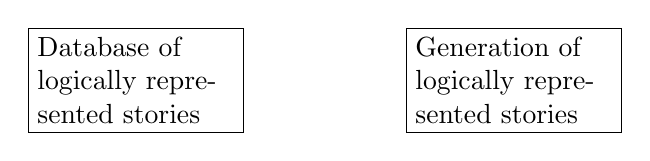
\begin{tikzpicture}
				\node[shape=rectangle,draw=black,text width=2.5cm] (logicdb) at (2*\myspacing,0) {Database
				of logically represented stories};
				\node[shape=rectangle,draw=black,text width=2.5cm] (logicgen) at (4*\myspacing,0) {
				Generation of logically represented stories};
			\end{tikzpicture}\\
		};
		\node[outer,draw=yellow,fill=yellow!20] (synopsis) at (0,-7) {
			\textit{Synopsis level}
			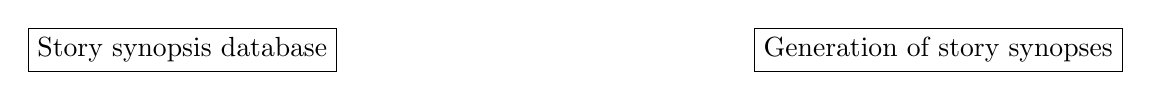
\begin{tikzpicture}
				\node[shape=rectangle,draw=black] (synopsisdb) at (\myspacing,0) {Story
				synopsis database};
				\node[shape=rectangle,draw=black] (synopsisgen) at (5*\myspacing,0)
				{Generation of story synopses};
			\end{tikzpicture}\\
		};
		\node[outer,draw=green,fill=green!20] (story) at (0,-10.5) {
			\textit{Story level}
			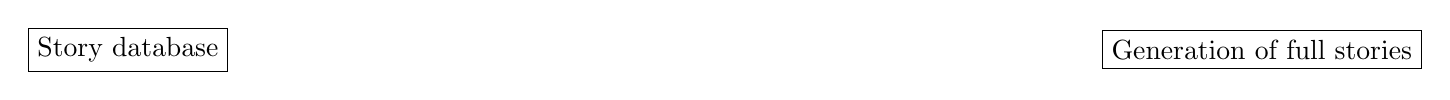
\begin{tikzpicture}
				\node[shape=rectangle,draw=black] (storydb) at (0,0) {Story
				database};
				\node[shape=rectangle,draw=black] (storygen) at (6*\myspacing,0)
				{Generation of full stories};
			\end{tikzpicture}\\
		};
		\draw[-{Stealth[scale=3.0]}] (storydb) -- (synopsisdb);
		\draw[-{Stealth[scale=3.0]}](synopsisdb) -- (logicdb);
		\draw[-{Stealth[scale=3.0]}](logicdb) -- (ruledb);
		\draw[-{Stealth[scale=3.0]}](ruledb) -- (logicgen);
		\draw[-{Stealth[scale=3.0]}](logicgen) -- (synopsisgen);
		\draw[-{Stealth[scale=3.0]}](synopsisgen) -- (storygen);
	\end{tikzpicture}
	\caption{The story generation pipeline}
	\label{storypipeline}
\end{figure}

The focus of this thesis is twofold: the main contribution is a way to extract
the story rules from a set of logically represented stories, and represent them 
in such a way that a program can be designed that can reason about these rules in a creative way. 
This corresponds to the logic database component at the top
of figure \ref{storypipeline}, which details the assumed pipeline. To do this, the story synopses have been
annotated manually to be able to focus on this part. However, the story
representation has been chosen in such a way that it could plausibly be extracted
in that form through natural language processing. 
This story annotation scheme is another contribution of this thesis. Its
simplicity makes it easy to annotate (and later, to extract the story structure automatically),
easy to visualize (which is important if this system is going to be used as a
co-creator with a human author) and easy to reason on (it is easy to find the
difference between different story states).
%TODO mention where potential uses are discussed

The overall approach of the work described in this thesis is as follows: the
stories are assumed to be annotated as a sequence of story states (represented
as graphs of characters, their goals and desires, and how these interact with
each other) and actions (simple sentences in natural language describing story
events). First, the action sentences are parsed to find the object, subject,
verb and dative (where applicable). Then, the preconditions of the actions (what
has to be true before this event can occur?) and the effects of the action (what
happens when this even takes place in the story?) are extracted, by looking at
the states prior and following the event. This information is then stored in a
database, which can be queried to obtain the likelihood of particular events.

\subsection{Story representation}

Before the rule extraction process will be covered, the story representation
will be discussed, since this influenced the representation of the rules.
A basic story is represented by a series of states $s_i$ and actions $a_j$.
Each story starts in some initial state $s_0$, then one or more actions happen
($a_0, ..., a_j$). These actions involve at least one, but
possibly multiple characters in the story, and transform the story state $s_0$
into $s_1$. This is followed by one or more actions
again, which leads to $s_2$, and so on. This pattern continues until the final 
state of the story, which is where the story ends. This model is inspired by the
MEXICA model, although it is less constrained, since a state can be followed by
multiple actions instead of just one.

The story sequence is assumed to be represented temporally ($s_{i+1}$ occurs
after $s_i$). To represent events happening in parallel, stories can contain
stories themselves too. For example, in a story, character A meets
character B at some place, and character B will tell character A about the
events that led character B to be at this particular place. Such a flashback
does not usually involve character A, and therefore can be considered a story within a
story. Another set of examples of stories where this construction would be
useful would be the stories of `One Thousand and One Nights' or `Canterbury Tales',
which are framing stories containing stories themselves. For the current algorithm, this construction does not
affect the rule extraction (the stories are read as separate stories), 
but for future deeper analysis this construction could be useful. If story
structure will also be learned from existing stories, this might be helpful to a
program that has to be able to generate flashbacks or framing stories, since it
enables stories to serve as examples of self-contained narratives (meaning that
the story-within-a-story has to be finished before the main story resumes).

\begin{figure}
	\begin{tikzpicture}[remember picture,
		outer/.style={draw=blue,fill=blue!20,thick,inner sep=10pt}
	]
		\node[outer,draw=blue] (s1) at (0,0) {
			\begin{tikzpicture}
				\node[shape=rectangle,draw=black] (1p) at (0,0) {princess};
				\node[shape=rectangle,draw=black] (1pac) at (3.5,2) {princess\_abilities:companionship};
				\node[shape=rectangle,draw=black] (1pnb) at (3.5,-2) {princess\_needs:retrieve(ball)};
				\node[shape=rectangle,draw=black] (1pr1) at (7,0.75) {promise:1};
				\node[shape=rectangle,draw=black] (1pr2) at (7,-0.75) {promise:2};
				\node[shape=rectangle,draw=black] (1fab) at (10.5,2) {frog\_abilities:get(ball)};
				\node[shape=rectangle,draw=black] (1fnc) at (10.5,-2) {frog\_needs:companionship};
				\node[shape=rectangle,draw=black] (1f) at (15,0) {frog};

				\draw[-] (1p) -- (1pac);
				\draw[-] (1p) -- (1pnb);
				\draw[-] (1pac) -- (1pr1) -- (1fnc);
				\draw[-] (1pnb) -- (1pr2) -- (1fab);
				\draw[-] (1fab) -- (1f);
				\draw[-] (1fnc) -- (1f);
			\end{tikzpicture}\\
			\textit{State 1}
		};
		\node[shape=rectangle,draw=black] (a1) at (0, -4) {the frog gets the ball};
		\node[outer,draw=blue] at (0,-8) (s2) {
			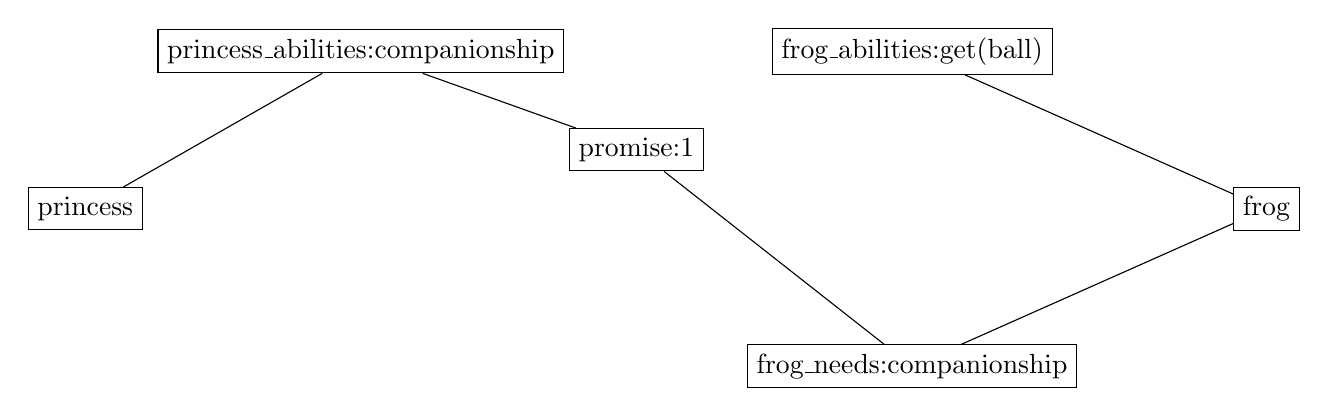
\begin{tikzpicture}
				\node[shape=rectangle,draw=black] (2p) at (0,0) {princess};
				\node[shape=rectangle,draw=black] (2pac) at (3.5,2) {princess\_abilities:companionship};
				\node[shape=rectangle,draw=black] (2pr1) at (7,0.75) {promise:1};
				\node[shape=rectangle,draw=black] (2fab) at (10.5,2) {frog\_abilities:get(ball)};
				\node[shape=rectangle,draw=black] (2fnc) at (10.5,-2) {frog\_needs:companionship};
				\node[shape=rectangle,draw=black] (2f) at (15,0) {frog};

				\draw[-] (2p) -- (2pac);
				\draw[-] (2pac) -- (2pr1) -- (2fnc);
				\draw[-] (2fab) -- (2f);
				\draw[-] (2fnc) -- (2f);
			\end{tikzpicture}\\
			\textit{State 2}
		};
		\draw[-] (s1) -- (a1) -> (s2);
	\end{tikzpicture}
	\caption{Representation of a simple state-action-state transition.
	\textit{State 1}
	represents the part of ``The Frog Prince'' where the frog had promised to get
	the princess's golden ball from the bottom of a pond, in return for spending
	time with him (these promises are represented as relations between the
	relevant abilities and needs of the princess and the frog). There is one
	action, where the frog gets the ball for the princess, which leads to the
	altered state in \textit{State 2} (The princess does not need the ball
	anymore, and the promise has been fulfilled, which is why both nodes have
	been removed from the graph).}
	\label{storyrep}
\end{figure}

\subsubsection{States}

States are represented as a graph filled with nodes. These nodes represent currently
active characters, their abilities and their needs. The relations in the graph define a
connection between these entities. The state represents the existents in the
story, as defined by the Chatman model presented in the section 3, since
it contains the characters and objects (which could be seen as part of the
setting) that are active in the story at the time.
An example of two states can be seen in figure \ref{storyrep}.
In this figure we see the princess and frog characters represented as nodes,
their abilities and desires being nodes themselves that are connected to their
respective characters. 

Agreements such as promises are also represented as
nodes, connecting abilities and desires with eachother. For example,
`\texttt{promise:2}' in State 1 represents the frog's promise to get the ball for the
princess. This is because the node is connected to the node
\texttt{frog\_abilities:get(ball)} (representing the frog's ability to retrieve the
ball) and the node \texttt{princess\_needs:retrieve(ball)} (representing the princess
wanting to have the ball).

\subsubsection{Actions}

Actions are represented as a short, natural language-like phrase (for example 
\texttt{``the frog gets the ball"}
or \texttt{``the frog promises the ball to the princess"}). The action in this
model actually represents the event as defined in section 3, which
can be either an action (a deliberate action executed by a character) or a happening (events that
happen without being done intentionally by a character)
The actions were not annotated in the form of logic, since being able to parse actions in natural
language would be a step closer to the goal of both extracting patterns directly
from story synopses written in natural language and generating the synopsis of a
story in natural language from a logical representation. In other words, these
sentences are closer to the sentences which might be found in the story synopsis
database (component 2 of the pipeline outlined in section 4.1).
These sentences are parsed with the Python Natural Language Toolkit (NLTK)
\cite{BirdKleinLoper09}
to obtain the subject, verb and optionally the object and/or dative (which will be
referred to as $\texttt{subj}, \texttt{verb}, \texttt{obj}$ and $\texttt{dat}$,
respectively). For example "the frog gets the ball" would yield 
$\texttt{obj}=\textrm{``ball"}, \texttt{subj}=\textrm{``frog"},
\texttt{verb}=\textrm{``gets"}, \texttt{dat}=\textrm{``"} $. First the
sentences are tokenized (individual words are separated, comma's are separated
from the word they are attached to, etc.). Then NLTK assigns a
Part of Speech (P.O.S.) tag, denoting the lexical category that the word belongs
to. This takes care of the ambiguity found on the lexical level by looking at
the context in which the word appears (in the second example, ``promises" could
be a noun or a verb, but due to the context it is tagged as a verb). For the
experiments the P.O.S.-tagger recommended by the NLTK was used, which is a perceptron tagger
trained on the Penn Treebank dataset.

Then, the sentence is parsed using a simple tree-parser which uses a feature-based
grammar. This grammar contains rules to infer which word is the subject, which
word is the object, and so on. The rules in the grammar have the following form:
$$
\texttt{S}{[}\texttt{subj}=s, \texttt{verb}=v, \texttt{obj}=o, \texttt{dat}=d{]}
\Rightarrow
\texttt{NP}{[}\texttt{N}=s{]} \texttt{VP}{[}\texttt{V}=v, \texttt{N}=o,
\texttt{dat}=d{]}
$$
On the left hand side there is one non-terminal (in this case $\texttt{S}$), and
on the right hand side there is at least one terminal or non-terminal symbol
($\texttt{NP}$ and $\texttt{VP}$). The values for the variables are obtained in
a recursive fashion. This means that the instantiation of $s$, $v$ and $o$ in
the previous rule are dependent on the rules
chosen to expand the $\texttt{NP}$ and $\texttt{VP}$ nodes of the tree. After
enough node expansions a non-terminal will be expanded to a terminal, which will
instantiate the variables. This way we obtain values for $\texttt{subj}$ 
$\texttt{obj}$ $\texttt{verb}$ and $\texttt{dat}$. It is imporant to note again that
not all of these fields need to be instantiated. Most sentences don't have a
dative, and with intransitive verbs there is no object either (for example, the
sentence `John walks.' only has a subject (`John') and a verb (`walks')).
An example of what happens if the sentence ``the frog gets the
ball'' is parsed can be seen in figure \ref{parse_example}.

\begin{figure}
	\Tree 
	[.{\texttt{S}{[}\texttt{subj}=\textrm{``frog''},
	\texttt{verb}=\textrm{``gets''}, \texttt{obj}=\textrm{``ball''},
	\texttt{dat}=\textrm{``''}{]}} 
		[.{\texttt{NP}{[}\texttt{N}=\textrm{``frog"}{]} }
			[.{\texttt{Det}{[}\texttt{Det}=\textrm{``the"}{]}} the ] 
			[.{\texttt{N}{[}\texttt{N}=\textrm{``frog"}{]}} frog ]
		] 
		[.{\texttt{VP}{[}\texttt{V}=\textrm{``gets"}, \texttt{N}=\textrm{``ball"}, \texttt{dat}=\textrm{``"}{]}}
			[.{\texttt{V{[}V=\textrm{``gets"}{]}}} gets ] 
			[.{\texttt{NP}{[}\texttt{N}=\textrm{``ball"}{]} }
				[.{\texttt{Det}{[}\texttt{Det}=\textrm{``the"}{]}} the ] 
				[.{\texttt{N}{[}\texttt{N}=\textrm{``ball"}{]}} ball ]
			]
		]
	]
	\caption{An example of an action being parsed from a sentence}
	\label{parse_example}
\end{figure}

By applying the grammar rules, the tree parser eventually finds the object, subject, verb
and dative of the sentence and store these variables, if they have been
instantiated. The extracted action looks as follows:

\begin{verbatim}
[ OBJ    = `ball' ]
[ SUB    = `frog' ]
[ VERB   = `gets' ]
\end{verbatim}

The dative is missing here, since this sentence lacks a dative.

\subsection{Rules}

When the actions have been extracted, the corresponding rule has to be
extracted. This means extracting the precondition (\texttt{prec}) and the effect
(\texttt{eff}) by looking at the state before the action happened and the state
after the action happened. These two concepts together represent the setting
rules as defined in section 3 and will be further explained in section 4.3.1. The source of the rule
is also stored in the \texttt{source} variable. This section will discuss the representation of the
rules, the extraction process and how the resulting rules are queried.

\subsubsection{Rule representation}

Rule objects are similar in form to action objects. These are extracted from 
the stories by seeing how states are affected by a certain action.
They are represented as a tuple of $(\texttt{action}, \texttt{obj}, \texttt{subj}, \texttt{dat}, \texttt{source},
\texttt{prec}, \texttt{eff})$. These concepts are defined as
follows:

\begin{itemize}
\item Here, the verb denoting which action is taking place is stored in 
$\texttt{action}$.
This is obtained from the parsed sentences's $\texttt{verb}$ field.
For example, ``promises'' is the action obtained from the
sentence \texttt{``the frog promises the ball to the princess''}, since
``promises'' is the verb of the sentence.

\item The representation also stores which agents
acted as objects, subjects, and datives in 
\texttt{obj}, \texttt{subj} and \texttt{dat}, respectively.
This is because the representation was developed for fairy tales, which often contain certain stock 
characters (the king, the princess, the witch, etc.). These characters often
fullfill the same kind of role across fairy tales (the prince marries the
princess in many stories, for example).
That way, the program
could for example learn that the princess character rarely murders anyone
(the princess acting as the subject of the `murder' action has a low probability), but
is more likely to marry someone (the princess acting as the subject of the
`marry' action has a high probability) or
be married by someone (the princess acting as the object of the `marry' action
has a high probability). How these probabilities are computed will be covered in
section 4.3.3.

\item \texttt{source} stores the name of the story from which the rule was extracted.
This could be used in a future generation system to look up what story the rule
is from, which could link this to the relevant text in the synopsis en the
relevant text in the full story. This could then be used in the generation
program to learn how to generate synopses from the logical representation, and
full stories from the synopses.

\item \texttt{prec} represents the preconditions of the action in terms of what 
relations certain actors should have with each other (in other words, what has
to be true in the current story state before this action becomes possible?).
This is represented as a reduced subset of the action directly prior to the
action, only involving the characters involved in the action, their properties
and the relations between each character.

\item \texttt{eff} represents the effects of the action (what
happens if this action is taken?). This is expressed in terms of either nodes in the
state graph appearing or dissappearing (these nodes can be characters, their
desires and abilities) or connections between nodes (representing the
connections between these entities) appearing or dissappearing.

For example, if $a = \texttt{"kill"}$, $\texttt{prec}$ might be 
$ \{\texttt{hates}(\texttt{subj}, \texttt{obj})\} $ (a character has to hate someone 
before they kill them), and $\texttt{eff}$ would be ${\texttt{delete}(\texttt{obj})}$
(if a character is killed, they are removed from the next state).
Note that both $\texttt{prec}$ and $\texttt{eff}$ are sets of conditions.
An action can have multiple prerequisites and multiple effects on the story state.

\end{itemize}

\subsubsection{Extracting rules}

Extracting the effect $\texttt{eff}$ of an action is the easiest. For now
actions are not assumed to have effects that do not become apparent immediately
(in other words, the action has an immediate effect on the next state, but no
lingering effects on the states after that).
Therefore it is enough to see what the difference is between the state before
and the state after the action. The different concepts that are tracked are the
nodes in the graph that appear and disappear in the new state, and the
connections that appear and dissappear in the new state.

However, because multiple actions can appear between states it is difficult to
discern which actions affects what parts of the network. 
Therefore, for each action, the algorithm only looks at the actors involved in 
the action ($\texttt{obj}, \texttt{subj}, \texttt{dat}$), and the nodes
connected to them directly (these nodes are assumed to be either desires or
abilities of the characters). This keeps the preconditions managable too, since
they don't just include the whole state difference, but only the relevant parts
for the action. Of course this assumption breaks down if a lot of actions
between two states
involve the same actor (making it unclear what action had what effect), but this pruning of possible actors does already reduce
the ambiguity in a meaningful way.

At first the program only looked at the characters themselves, but since the
interesting relations were mostly between the desires and abilities of the
characters, and not the characters themselves (for example, in figure
\ref{storyrep} there is no direct relation between the princess and frog nodes,
but their abilities and desires are linked to promises), this did not pick up the more
interesting preconditions and effects of each action.

Consequently, in figure \ref{storyrep} the frog node and the nodes containing the word
"ball" ("frog\_abilities:ball" and "princess\_needs:ball") are considered by the
program, as
well as their immediate neighbor nodes and the connections to them (in effect,
the whole first state excluding the princess node).

Similar to effects, for the preconditions $\texttt{prec}$ the state immediately prior to the action
is assumed to have all the
necessary information for the action in it (it is not necessary to look at the 
preceding states, since they offer no additional information). Therefore all
information in the previous state is assumed to be a part of the precondition.
This is analogous to the Markov property found in Markov chains, where the
previous state also contains all necessary information to predict the
next action that has to be taken.
However, this is reduced like the preconditions to only the actors involved in
the action, and the nodes directly connected to them.

Another context unit that is also stored is in which story a particular occurence of a
rule was found. This can later be helpful if the program is used as a tool for
story analysis (since one can easily see where a rule comes from, and which
stories have similar rule structures), but could also be used to guide the creation process of a
generation algorithm, by introducing a bias for certain stories if so desired.
This bias would be helpful if the program would be allowed to train on stories
it generated itself, giving preference to human-created stories, since they are
known to be well-constructed.

Before storing the preconditions and effects, all occurences of the characters
in these rules are substituted for variables.
This is
done so that rules can be more easily compared, since for rule analysis the
function a character has in the event is more important than the character
archetype. Without this step an extra
lookup of the character's function in a rule could be done whenever the rule 
is queried, but it is easier to only do this once.
This is done by seeing which
characters are involved in what function ($\texttt{obj}, \texttt{subj}, \texttt{dat}$)
and substituting them for a variable denoting this function. In the example, the
subject \texttt{subj} equals `frog', so all occurences in the preconditions and
effects of the term `frog' are substituted for the variable `SUB'.
Given the action parse of the previous section and the states present in figure
\ref{storyrep}, the following rule is extracted.

\begin{verbatim}
OBJ = `ball'
SUB = `frog'
PREC = [
    (`SUB', `SUB_abilities:get(OBJ)'),
    (`SUB_needs:companionship', `promise:2'),
    (`SUB_needs:companionship', `SUB'),
    (`SUB', `SUB_race:animal'),
    (`SUB_abilities:get(OBJ)', `promise:1'),
    (`SUB_abilities:get(OBJ)', `SUB'),
    (`SUB', `SUB_needs:companionship'),
    (`SUB_race:animal', `SUB')
    ]
EFF = {
    `edges_gone': [
        (`promise:1', `SUB_abilities:get(OBJ)')
        ]
    }
SOURCE = `frogprince'

\end{verbatim}

\subsubsection{Obtaining rule probabilities}

All extracted actions are stored together in a database (in the current
implementation this is a Python dictionary, with the actions as keys and the
rest of the information stored in an object as a value). This database can be
queried for the probabilities of certain actions: 
$$p(a) = \frac{\it{Count}(a)}{\sum_{x \in A}\it{Count}(x)}$$
Here $a$ is the action and $A$ is the set of all seen actions.
This database can also be queried in a conditional manner (for
example, if a generation program needs to find some action for the princess to
perform in the story, we
can simply query the probability of different actions, given that the princess
is the subject of the action:
$$p(a \mid a_{\texttt{subj}}=\texttt{``princess''}) = 
\frac{\it{Count}(a \land a_{\texttt{subj}}=\texttt{``princess''})}{\it{Count}(a)}$$
In the current implementation, no probabilities are pre-calculated, but if this
system would be trained on a large amount of stories it would be better to
at least store the counts for all actions in a table to speed up the calculation
of the probabilities.

The rule probabilities can be used by a planning algorithm to generate stories in a
creative manner. In the introduction of this paper, we noted that for artistic
creativity, in this case story generation, we have to generate stories
that are both novel but are also comprehensible. With the action probabilities,
we have a metric of how plausible certain actions are, so a planning algorithm
could choose the next action based on how plausible the story is. If the story
is following the existing stories too much (the probability of the
generated story becomes too high), it can choose an action with a
low probability in an attempt to make the story more creative. But if the story becomes too
unpredictable (the probability of the story becomes too low), the program might
choose an action with a high probability to try to balance things out. However, finding
which exact values to use for the upper and lower boundaries for this algorithm
would require more annotated stories to do a proper analysis, and is therefore
outside the scope of this thesis.

\subsubsection{Using rule probabilities}

As we saw in section 4.3.2, rules contain the following information:
\begin{itemize}
\item \texttt{action}
\item \texttt{obj}
\item \texttt{subj} (optional)
\item \texttt{dat} (optional)
\item \texttt{prec}
\item \texttt{eff}
\item \texttt{source}
\end{itemize}

Essentially, probabilities can be computed for the occurence of every variable
in the rule object, and for every combination of rule object variables. Some
interesting possibilities are:

\begin{itemize}
\item \textbf{Comparison between action and obj, subj or dat:} This way a
generation program can obtain the knowledge of how characters interact with the
action (for example, the probability that a princess will marry is high, the
probability that a princess will murder someone is low (
$p(\texttt{action}=\texttt{``marry''} \mid \texttt{subj}=\texttt{``princess''}) \gg
p(\texttt{action}=\texttt{``murder''} \mid \texttt{subj}=\texttt{``princess''})
$))
\item \textbf{Comparisons between the different obj, subj and dat of the same
action:}
For example, character X (the prince) and character Y (the caliph) are often the subject of the
same action A (marriage) (in probabilistic terms
$p(\texttt{subj}=\texttt{``prince''} \mid \texttt{action}=\texttt{``marry''})
\approx
p(\texttt{subj}=\texttt{``caliph''} \mid \texttt{action}=\texttt{``marry''})$
). Perhaps these characters are similar to each other
(they fulfill the same type of function in stories) and could be substituted in
the same action (if the prince usually marries a princess, perhaps a caliph
could also marry a princess) or different actions (if the prince has a high
probability of slaying dragons, the caliph might also be able to slay dragons,
even if it has never been seen before).
\item \textbf{Comparison between combinations of obj, subj, dat over different actions:}
Another option would be to see which characters are connected, by seeing which
characters often appear in the same actions. For example, princes and princesses
frequently interact with eachother (across different actions such as one saving
the other, marrying, etc.). This is true if \\
$p(
	(\texttt{subj}=\texttt{``prince''} \land \texttt{obj}=\texttt{``princess''})
	\lor \\
	(\texttt{subj}=\texttt{``princess''} \land \texttt{obj}=\texttt{``prince''})
	\lor \\
	(\texttt{subj}=\texttt{``prince''} \land \texttt{dat}=\texttt{``princess''})
	\lor \\
	(\texttt{subj}=\texttt{``princess''} \land \texttt{dat}=\texttt{``prince''})
	\lor \\
	(\texttt{obj}=\texttt{``prince''} \land \texttt{dat}=\texttt{``princess''})
	\lor \\
	(\texttt{obj}=\texttt{``princess''} \land \texttt{dat}=\texttt{``prince''})
)$ is higher than some threshold or higher than other character combinations.

This indicates that these characters often appear together, which might be 
useful when a future generation program needs to select
new characters to introduce in a story (the reasoning being `There is already a
princess in the story, it would make sense to introduce a prince character.').
This character selection process is important if the generation program needs to
be able to make certain events happen (There can not be a marriage between the
prince and the princess if either one of these characters is missing).
\end{itemize}
